\documentclass[13pt,oneside, aspectratio=169]{beamer}
\usepackage[utf8]{vietnam}
%\usepackage[linesnumbered, commentsnumbered]{algorithm2e}
\usepackage{appendixnumberbeamer}
\usepackage{multirow}
\usepackage{makecell}
\usepackage{verbatim}


\usepackage[sorting=none,style=numeric,backend=bibtex]{biblatex}
\bibliography{reflib.bib}
%\usepackage{beamerthemesplit} 
\setbeamertemplate{footline}[frame number]
\setbeamertemplate{headline}{}
\usepackage{pgfplots}
\pgfplotsset{compat=newest}
\usepackage{booktabs}
%%%%%%%%%%%%%%%%%%
\definecolor{CTUcyan}{rgb}{0, 0.6862745098039216, 0.9372549019607843}
\definecolor{CTUblue}{rgb}{0.121568627450, 0.3607843137254902, 0.6627450980392157}

\usepackage{amsfonts,amsmath,amssymb,mathptmx,times}
\usepackage{algorithm}
\usepackage{algorithmicx}
\usepackage{verbatim}
\usepackage{graphicx}
\usepackage{subcaption}
\usepackage{booktabs,multicol,calligra}  %Allows the use of \toprule, \midrule and \bottomrule in tables
\usepackage{hyperref}
\usepackage{tcolorbox}
\usetikzlibrary{arrows,shapes}
\usepackage{multicol}
\usepackage{animate}



\mode<presentation>
{
	
	\setbeamertemplate{background canvas}{
		\begin{tikzpicture}
			\path (0,0) -- (\paperwidth,\paperheight);
			\node[opacity=.1] at (0.5\paperwidth,0.45\paperheight)
			{
\includegraphics[width=6cm]{BG/CTU_logo_singlecolor}};
		\end{tikzpicture}
	}
	
	\useinnertheme[shadow]{rounded}
	\useinnertheme{circles}
	\setbeamertemplate{navigation symbols}{}
	\setbeamertemplate{caption}[numbered]
	\setbeamercolor*{palette tertiary}{use=structure,bg=CTUblue}
	\setbeamercolor*{palette quaternary}{fg=white,bg=CTUblue}
	\setbeamercolor{frametitle}{fg=CTUblue}
	\setbeamercolor{title}{fg=CTUblue}
	
	\setbeamercolor{block title}{bg=CTUblue, fg=white}
	\setbeamerfont*{frametitle}{size=\Large,
		series=\bfseries,
		parent=structure}
	\setbeamercolor{block body}{bg=CTUblue!10}
	\setbeamercolor{section in toc}{fg=white}
	\setbeamercolor{subsection in toc}{fg=white}
	%	
}



\beamertemplatenavigationsymbolsempty




%\titlegraphic{
	%	\includegraphics[width=1cm]{Logo Đại Học Văn Lang H.png}
	%}
\title[]{\textbf{Nhận dạng thống kê cho hàm mật độ xác suất mất~cân~bằng và ứng dụng cho ảnh}}
\subtitle{Báo cáo đề cương bảo vệ luận văn tốt nghiệp thạc sĩ}
\author[HUNG Tran-Nam]{Trần Nam Hưng\inst{1}}
\institute[CTU]{
	\inst{1} Khoa Khoa học Tự nhiên, Trường Đại học Cần Thơ
}

\date[Oct 20, 2024]{Ngày 20 tháng 10 năm 2024}

%\AtBeginSection[ ]
%{	
%	\usebackgroundtemplate{
\includegraphics[width=\paperwidth]{BG/thank2.pdf}}%
%			\begin{frame}
%						{\Large\bf\color{white} Mục lục}}
%						\tableofcontents[currentsection]
%					\end{frame}
%		}


\begin{document}
	
	{
		\usebackgroundtemplate{
\includegraphics[width=\paperwidth]{BG/background.pdf}}%
		\begin{frame}[plain]
			\vspace{2cm}
			\titlepage
		\end{frame}
	}
	
	{
		\usebackgroundtemplate{
\includegraphics[width=\paperwidth]{BG/thank2.pdf}}%
		
		
		\begin{frame}{}
			\vspace{3em}
			{\Large\bf\color{white} Mục lục}
			\large\color{white} \tableofcontents
		\end{frame}
	}










	
	\section{Phần mở đầu}
	
%	\begin{frame}{1. Lý do chọn đề tài}{Nghiên cứu – phát triển các nguyên tắc và ứng dụng hệ thống thông minh nhân tạo (AI) là yếu tố then chốt nhằm thúc đẩy tăng trưởng kinh tế bền vững ở các quốc gia}
%		
%\end{frame}
	
		\begin{frame}{1. Lý do chọn đề tài}{Nhận dạng thống kê gồm có hai bài toán chính \cite{Bishop:DeepLearning24,webb2003statistical,theodoridis2006pattern}}
			Trong sự phát triển của AI, nhận dạng thống kê được xem là một trong những kiến thức nền tảng.
			\begin{figure}
				\centering
			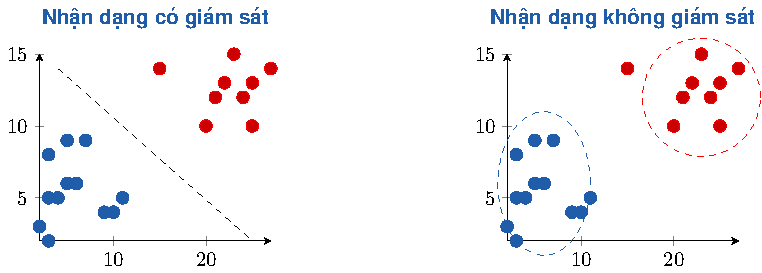
\includegraphics[width=.9\linewidth]{ML}
		\end{figure}
		
	\end{frame}
	
		\begin{frame}{1. Lý do chọn đề tài}{Nhận dạng thống kê cho hàm mật độ xác suất được đề xuất \cite{nguyen2024new,nguyentrang2017fuzzy}}
				\begin{figure}
		\centering
		\subfloat[\centering CDE: $k$-mean, FCM, PCM, DBSCAN]{{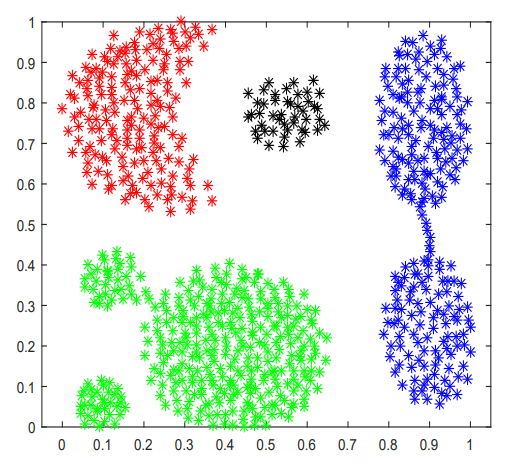
\includegraphics[width = 0.22\linewidth]{image/CDE}}}
		\quad
		\subfloat[\centering CDI]{{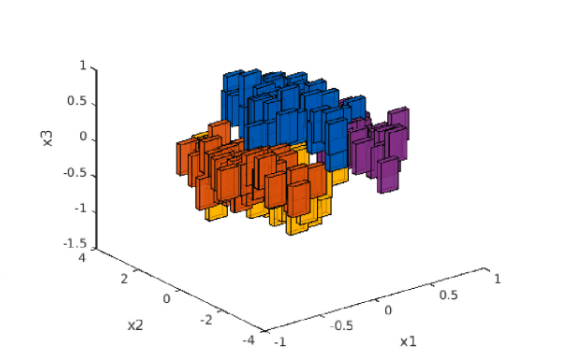
\includegraphics[width = 0.32\linewidth]{image/CDI}}}
		\qquad
		\subfloat[\centering {\color{blue} \bf CDF}: SUF, automatic]{{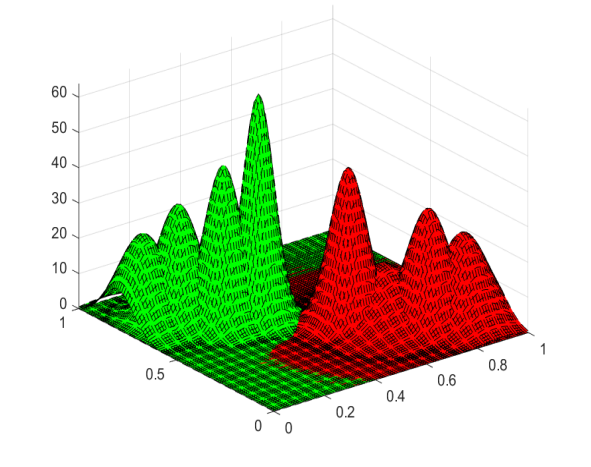
\includegraphics[width = 0.28\linewidth]{image/CDF}}}
		\quad
		\subfloat[\centering {\color{blue} $\ldots$}]
		\quad
	\end{figure}
	
	
 	\end{frame}
	
			\begin{frame}{1. Lý do chọn đề tài}{Trong nhận dạng dữ liệu thực tế, cần thiết xử lý tình trạng dữ liệu mất cân bằng \cite{tang2008svms,hu2024gat}}
		\begin{figure}
			\centering
			
\includegraphics[width=\linewidth]{image/iB}
		\end{figure}
		Nhận dạng thống kê dữ liệu mất cân bằng cho hàm mật độ xác suất cần được quan tâm.
	\end{frame}
	
	
	
		\begin{frame}{2. Mục đích nghiên cứu}
		\begin{itemize}
			\item \textbf{Xây dựng thuật toán} phân loại và phân tích chùm cho hàm mật độ xác suất với dữ liệu
			mất cân bằng;
			\item\textbf{Áp dụng cho dữ liệu ảnh} khi các đặc trưng của nó được trích xuất và
			đại diện bởi PDF để nhận dạng.
		\end{itemize}
	\end{frame}
	
	\begin{frame}{3. Đối tượng và phạm vi nghiên cứu}
		\begin{enumerate}
		\item \textbf{Đối tượng nghiên cứu}
		\begin{itemize}
			\item Thuật toán phân loại và phân tích chùm với dữ liệu mất cân bằng;
			\item Dữ liệu ảnh được trích xuất thành các đối tượng đại diện.
		\end{itemize}
		\item\textbf{Phạm vi nghiên cứu}
		\begin{itemize}
			\item Các thuật toán phân tích chùm và phân loại chỉ cho PDF;
			\item Dữ liệu ảnh được trích xuất thành PDF đại diện;
			\item Vấn đề tính toán của các phương pháp phân loại, phân tích chùm.
		\end{itemize}
		\end{enumerate}
	\end{frame}
	
	
	\begin{frame}{4. Phương pháp nghiên cứu}
		\begin{itemize}
			\item \textbf{Nghiên cứu lý thuyết:} Phân tích, tổng kết, phân loại, hệ thống hóa kiến thức; So sánh đánh giá 
			\item \textbf{Thực nghiệm khoa học:} Thực hiện các ví dụ số; xử lý so sánh kết quả
		\end{itemize}
	\end{frame}
	
	\section{Nội dung nghiên cứu}
	
	\begin{frame}{Cấu trúc luận văn}
	\begin{figure}
		\centering
		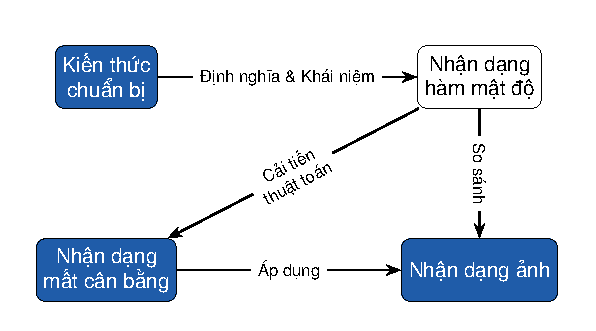
\includegraphics[width=.9\linewidth]{mindchart}
	\end{figure}
	\end{frame}
	
	
	
	
	\section{Phần kết luận}
	
	\begin{frame}{Phần kết luận}
		\begin{itemize}
			\item Tổng kết các vấn đề đã thực hiện trong đề cương;
			\item Đánh giá những khó khăn, hạn chế của các mô hình về mặt lý thuyết và ứng dụng;
			\item Đưa ra những định hướng có thể phát triển trong thời gian tới từ những nghiên cứu đã
			thực hiện.
			\end{itemize}
	\end{frame}
	
	
	
	
	
	
	\section{Thời gian làm luận văn}

	\begin{frame}{Thời gian làm luận văn}
	
\begin{figure}
	\centering
	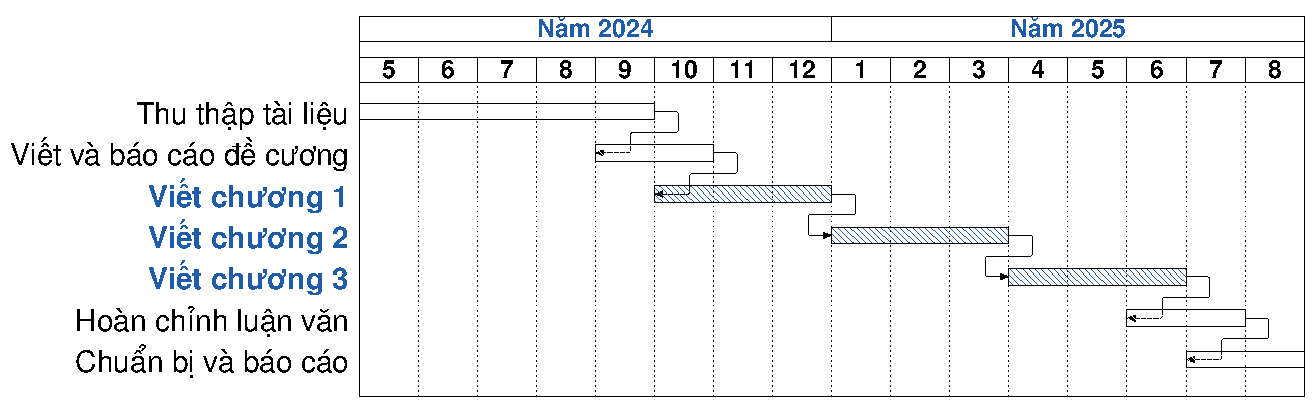
\includegraphics[width=\linewidth]{timeline}
\end{figure}

\end{frame}
	
	
	
	
	
	


	\section{Tài liệu tham khảo}
	
	
	\begin{frame}[allowframebreaks, noframenumbering]{Tài liệu tham khảo}\small
		\printbibliography
	\end{frame}
	

	
	

{
	\usebackgroundtemplate{
\includegraphics[width=\paperwidth]{BG/thank2.pdf}}%
	\begin{frame}
		\begin{center}\color{white}
			\vspace{1.2cm}
			
			{\Large\color{white}\bf Chân thành cảm ơn quý hội đồng!}
			
			
			\vspace{1cm}
			
			
				{\it A prudent question is one half of wisdom} --- F. Bacon
			

		\end{center}
		
		
	\end{frame}
}


%	{
%	\usebackgroundtemplate{
\includegraphics[width=\paperwidth]{BG/thank2.pdf}}%
%	
%	
%	\begin{frame}{}
%		\vspace{3em}
%		{\Large\bf\color{white} Mục lục}
%		\large\color{white} \tableofcontents
%	\end{frame}
%}




\end{document}